% !TEX TS-program = xelatex
% !TEX encoding = UTF-8 Unicode
% !Mode:: "TeX:UTF-8"

\documentclass{resume}
\usepackage{graphicx}
\usepackage{tabu}
\usepackage{multirow}
\usepackage{progressbar}
\usepackage{zh_CN-Adobefonts_external} % Simplified Chinese Support using external fonts (./fonts/zh_CN-Adobe/)
% \usepackage{NotoSansSC_external}
% \usepackage{NotoSerifCJKsc_external}
% \usepackage{zh_CN-Adobefonts_internal} % Simplified Chinese Support using system fonts
\usepackage{linespacing_fix} % disable extra space before next section
\usepackage{cite}
\usepackage{fontspec}

\usepackage{hyperref}
\hypersetup{
    colorlinks=true,
    linkcolor=blue,
    filecolor=blue,      
    urlcolor=blue,
    citecolor=cyan,
}

\begin{document}
\pagenumbering{gobble} % suppress displaying page number

\name{Xueyao Zhang(张雪遥)}

\basicInfo{
  \faHome{\href{https://www.zhangxueyao.com}{~~zhangxueyao.com}} \textperiodcentered\ 
  \faGraduationCap{\href{https://scholar.google.com/citations?user=lf1udBcAAAAJ&hl=en}{~~Google Scholar}} 
}

% \Large{
%   \begin{tabu}{ c l l }
%    \multirow{3}{1in}{
%        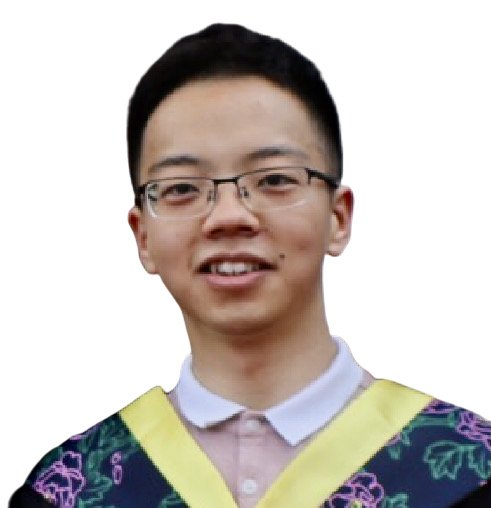
\includegraphics[width=0.95in]{me.jpeg}} & \scshape{Xueyao Zhang(张雪遥)} &  \\
%     % & \email{zhangxueyao19s@ict.ac.cn} & \phone{~~(+86) 152-0390-0168} \\
%     % & \phone{(+86) 152-0390-0168} &  \\
%     % & \faWechat{ xueyao\_98} & \github[~~github.com/RMSnow]{https://github.com/RMSnow} \\
%     & \faHome{\href{https://www.zhangxueyao.com}{~~zhangxueyao.com}}
%     & \faGraduationCap {\href{https://scholar.google.com/citations?user=lf1udBcAAAAJ&hl=en}{~~Google Scholar}} 
%   \end{tabu}
% }

\section{此PDF中所附论文如下:}
\textbf{
  \large Topic: \framebox[1.1\width]{Fake News Detection}
}

\datedsubsection{\textbf{1.} \quad \textit{\textbf{Mining Dual Emotion for Fake News Detection} (Long Paper; Oral; First-authored)}}{}
{\small \role{\textbf{\underline{Xueyao Zhang}}, Juan Cao, Xirong Li, Qiang Sheng, Lei Zhong, Kai Shu.}{Proceedings of the 30th Web Conference \textbf{(WWW 2021)}\quad \href{https://www.zhangxueyao.com/data/www2021-dual-emotion-paper.pdf}{[PDF]} \href{https://github.com/RMSnow/WWW2021}{[Code]} \href{https://www.zhangxueyao.com/data/www2021-dual-emotion-slides.pdf}{[Slides]} \href{https://www.zhangxueyao.com/data/www2021-dual-emotion-video.mp4}{[Video]} \href{https://www.bilibili.com/video/BV13o4y1m7c3}{[Chinese Video]}
}
\small
\textit{TL;DR}: We leverage both publisher emotion and social emotion for fake news detection.

\datedsubsection{\textbf{2.} \quad \textit{\textbf{Integrating Pattern- and Fact-based Fake News Detection via Model Preference Learning} (Long Paper; Oral; Co-first-authored)}}{}
{\small \role{Qiang Sheng*, \textbf{\underline{Xueyao Zhang}}*, Juan Cao, Lei Zhong. (*: Equal Contribution)}{Proceedings of the 30th ACM International Conference on Information and Knowledge Management \textbf{(CIKM 2021)}\quad \href{https://dl.acm.org/doi/10.1145/3459637.3482440}{[PDF]} \href{https://www.zhangxueyao.com/data/cikm2021-PrefFEND-poster.pdf}{[Poster]} \href{https://github.com/ICTMCG/Pref-FEND}{[Code]} \href{https://zhuanlan.zhihu.com/p/414464291}{[Chinese Blog]}}
}
\small
\textit{TL;DR}: We propose a graph-based model preference learning framework to separately handle the pattern and fact indicators in fake news detection.

\datedsubsection{\textbf{3.} \quad \textit{\textbf{Article Reranking by Memory-enhanced Key Sentence Matching for Detecting Previously Fact-checked Claims} (Long Paper; Poster; Second-student-authored)}}{}
{\small \role{Qiang Sheng, Juan Cao, \textbf{\underline{Xueyao Zhang}}, Xirong Li, Lei Zhong.}{Proceedings of the Joint Conference of the 59th Annual Meeting of the Association for Computational Linguistics \textbf{(ACL 2021)}\quad \href{https://aclanthology.org/2021.acl-long.425.pdf}{[PDF]} \href{https://www.zhangxueyao.com/data/acl2021-MTM-poster.pdf}{[Poster]} \href{https://github.com/ICTMCG/MTM}{[Code]} \href{https://zhuanlan.zhihu.com/p/393615707}{[Chinese Blog]}}
\small
\textit{TL;DR:} We detect previously fact-checked claims by matching them against the key sentences in fact-checking articles.

\textbf{\\ \large Topic: \framebox[1.1\width]{Automatic Music Creation}}
\datedsubsection{\textbf{1.} \quad \textit{\textbf{Structure-Enhanced Pop Music Generation via Harmony-Aware Learning} (Long Paper; First-authored)}}{}
{\small \role{\textbf{\underline{Xueyao Zhang}}, Jinchao Zhang, Yao Qiu, Li Wang, Jie Zhou.}{\textbf{(Under Review)}\quad \href{https://arxiv.org/pdf/2109.06441.pdf}{[Preprint]}}
}
\small
\textit{TL;DR}: We propose to learn harmony for generating form- and texture- enhanced pop music.

\end{document}
